\documentclass{standalone}
\usepackage{tikz}
\usetikzlibrary{arrows.meta, positioning, calc}

\begin{document}

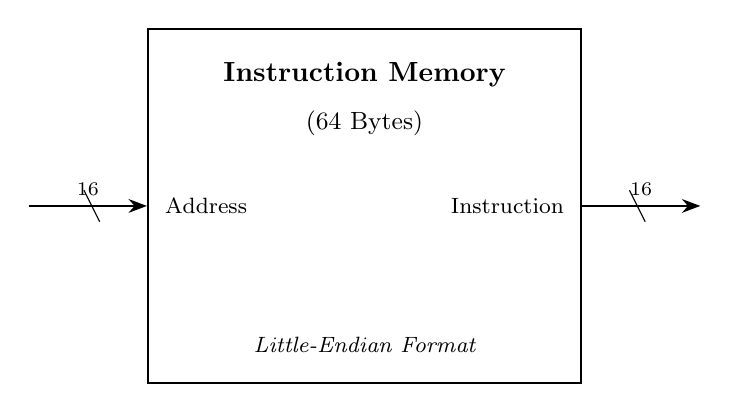
\begin{tikzpicture}[
    box/.style={rectangle, draw, minimum width=5.5cm, minimum height=4.5cm, thick, fill=white},
    port/.style={font=\footnotesize},
    label/.style={font=\scriptsize},
    arrow/.style={->, >=Stealth, thick}
]

    % Main Box
    \node[box] (mem) at (0,0) {};
    
    % Header Section: Title and Capacity
    \node[font=\bfseries, yshift=-0.6cm] (title) at (mem.north) {Instruction Memory};
    \node[font=\small, below=0.05cm of title] {(64 Bytes)};

    % Footer Section
    \node[font=\itshape\footnotesize, yshift=0.5cm] at (mem.south) {Little-Endian Format};

    % --- Left Side Input ---
    
    % Read Address
    \draw [arrow] ($(mem.west)+(-1.5, 0)$) -- ($(mem.west)+(0, 0)$)
        node[midway, above, label] {16}
        node[pos=1, anchor=west, port, xshift=0.1cm] {Address};
        
    % Bus Slash
    \draw ($(mem.west)+(-0.8, 0.2)$) -- ($(mem.west)+(-0.6, -0.2)$);

    % --- Right Side Output ---
    
    % Instruction Output
    \draw [arrow] ($(mem.east)+(0, 0)$) -- ($(mem.east)+(1.5, 0)$)
        node[midway, above, label] {16}
        node[pos=0, anchor=east, port, xshift=-0.1cm] {Instruction};
        
    % Bus Slash
    \draw ($(mem.east)+(0.6, 0.2)$) -- ($(mem.east)+(0.8, -0.2)$);

\end{tikzpicture}

\end{document}